\documentclass[a4paper,12pt]{article}

\usepackage{amsmath}
\usepackage[margin = 1in]{geometry}
\usepackage{graphicx}
\usepackage{booktabs}
\usepackage{natbib}

\usepackage{lipsum}
\usepackage[colorlinks = true,citecolor = blue]{hyperref}


\title{My First Stat Paper}
\author{Jerry Xu\\
Department of Statistics\\
University of Connecticut
}


\begin{document}
\maketitle
\section{Math Expression and Equation}
\begin{enumerate}\label{exp1}
    \item Here is the expression of natural basis of $e$
    \begin{align} e^{i\pi}+1=0 \end{align} Equation \ref{exp1} shows the relation between $e$ and integer.
    \item  But we can express it as:
    \begin{align}e = \lim_{n\to\infty}\left(1+\frac{1}{n}\right)^n\\ = \lim_{n\to\infty}\left(t+1\right)^{\frac{1}{t}}\end{align}
    \item  We can also express as:
     $e$ as \begin{equation}e = \sum_{n=0}^{\infty}\frac{1}{n!}\end{equation}
\end{enumerate}

\section{Table}
\begin{table}[!htbp] \centering 
  \caption{Statistical Summary of Several Distributions} 
  \label{} 
\begin{tabular}{@{\extracolsep{5pt}}lccccc} 
\\[-1.8ex]\hline 
\hline \\[-1.8ex] 
Statistic & \multicolumn{1}{c}{N} & \multicolumn{1}{c}{Mean} & \multicolumn{1}{c}{St. Dev.} & \multicolumn{1}{c}{Min} & \multicolumn{1}{c}{Max} \\ 
\hline \\[-1.8ex] 
normal & 10 & 0.152 & 0.655 & $-$1.330 & 0.779 \\ 
poisson & 10 & 3.600 & 2.459 & 0 & 8 \\ 
gamma & 10 & 4.302 & 3.005 & 1.298 & 9.980 \\ 
\hline \\[-1.8ex] 
\end{tabular} 
\end{table} 

\section{Figure}
This is where the plot come from \cite{zhang2003time}.
\bibliographystyle{plain}
\bibliography{reference}

\begin{figure}
    \centering
    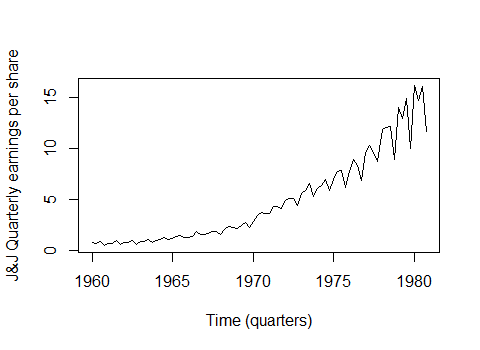
\includegraphics{tplt1.png}
    \caption{Time Series Plot for Quarterly Sales}
\end{figure}

\end{document}

